%\documentclass[a4paper,11pt,fleqn,oneside, openright]{memoir} % Brug openright hvis chapters skal starte p� h�jresider; openany, oneside

%%%% PACKAGES %%%%

% �� Overs�ttelse og tegns�tning �� %
\usepackage[utf8]{inputenc}					% G�r det muligt at bruge �, � og � i sine .tex-filer
\usepackage[danish]{babel}							% Dansk sporg, f.eks. tabel, figur og kapitel
\usepackage[T1]{fontenc}								% Hj�lper med orddeling ved �, � og �. S�tter fontene til at %v�re ps-fonte, i stedet for bmp	
\usepackage{latexsym}										% LaTeX symboler
\usepackage{xcolor,ragged2e,fix-cm}			% Justering af elementer
\usepackage{pdfpages}										% G�r det muligt at inkludere pdf-dokumenter med kommandoen \includepdf[pages={x-y}]{fil.pdf}	
\pretolerance=2500 											% G�r det muligt at justre afstanden med ord (h�jt tal, mindre orddeling og mere space mellem ord)
\usepackage{ulem}                       % Gennemstregning af ord med koden \sout{}
\usepackage{fixltx2e}										% Retter forskellige bugs i LaTeX-kernen
\usepackage{gensymb}					%Tilføjer \celsius og \degree notation	
\usepackage{lineno}						%Bruges til at tilføje linjetal
																	
% �� Figurer og tabeller � floats  �� %
\usepackage{flafter}										% S�rger for at dine floats ikke optr�der i teksten f�r de er sat ind.
\usepackage{multirow}                		% Fletning af r�kker
\usepackage{hhline}                   	% Dobbelte horisontale linier
\usepackage{multicol}         	        % Fletning af kolonner
\usepackage{colortbl} 									% Mulig�re farver i tabeller
%\usepackage{float}												% G�r det muligt at placere figurer hvor du vil.   \begin{figure}[!h] % Will not be floating.
\usepackage{wrapfig}										% Inds�ttelse af figurer omsv�bt af tekst. \begin{wrapfigure}{Placering}{St�rrelse}
\usepackage{graphicx} 									% Pakke til jpeg/png billeder
\pdfoptionpdfminorversion=6							% Muligg�r inkludering af pdf dokumenter, af version 1.6 og h�jere
	
% �� Matematiske formler og maskinkode ��
\usepackage{amsmath,amssymb,stmaryrd} 	% Bedre matematik og ekstra fonte
\usepackage{textcomp}                 	% Adgang til tekstsymboler
\usepackage{mathtools}									% Udvidelse af amsmath-pakken. 
\usepackage{eso-pic}										% Tilf�j billedekommandoer p� hver side
\usepackage{lipsum}											% Dummy text \lipsum[..]
\usepackage{rsphrase}										% Kemi-pakke til RS-s�tninger
\usepackage[version=3]{mhchem} 					% Kemi-pakke til lettere notation af formler

% �� Referencer, bibtex og url'er �� %
\usepackage{url}												% Til at s�tte urler op med. Virker sammen med hyperref
\usepackage[danish]{varioref}						% Giver flere bedre mulighed for at lave krydshenvisninger
\usepackage{natbib}											% Litteraturliste med forfatter-�r og nummerede referencer
\usepackage{xr}													% Referencer til eksternt dokument med \externaldocument{<NAVN>}

% �� Floats �� %
%\let\newfloat\relax 										% Memoir har allerede defineret denne, men det g�r float pakken ogs�
%\usepackage{float}

\usepackage[footnote,draft,danish,silent,nomargin]{fixme}		% Inds�t rettelser og lignende med \fixme{...} Med final i stedet for draft, udl�ses en error 																															for hver fixme, der ikke er slettet, n�r rapporten bygges.

%%%% CUSTOM SETTINGS %%%%

% �� Marginer �� %
\setlrmarginsandblock{3.5cm}{2.5cm}{*}	% \setlrmarginsandblock{Indbinding}{Kant}{Ratio}
\setulmarginsandblock{2.5cm}{3.0cm}{*}	% \setulmarginsandblock{Top}{Bund}{Ratio}
\checkandfixthelayout 									% Laver forskellige beregninger og s�tter de almindelige l�ngder op til brug ikke memoir pakker

%	�� Afsnitsformatering �� %
\setlength{\parindent}{0mm}           	% St�rrelse af indryk
\setlength{\parskip}{4mm}          			% Afstand mellem afsnit ved brug af double Enter
\linespread{1,1}												% Linie afstand

% �� Litteraturlisten �� %
\bibpunct[,]{[}{]}{;}{a}{,}{,} 					% Definerer de 6 parametre ved Harvard henvisning (bl.a. parantestype og seperatortegn)
%\bibliographystyle{bibtex/harvard}			% Udseende af litteraturlisten. Ligner dk-apali - mvh Klein

% �� Indholdsfortegnelse �� %
\setsecnumdepth{subsection}		 					% Dybden af nummerede overkrifter (part/chapter/section/subsection)
\maxsecnumdepth{subsection}							% �ndring af dokumentklassens gr�nse for nummereringsdybde
\settocdepth{section} 								% Dybden af indholdsfortegnelsen

% �� Visuelle referencer �� %
\usepackage[colorlinks=true]{hyperref}			 	% Giver mulighed for at ens referencer bliver til klikbare hyperlinks. .. [colorlinks]{..}
\hypersetup{pdfborder = 0}							% Fjerner ramme omkring links i fx indholsfotegnelsen og ved kildehenvisninger ��
\hypersetup{														%	Ops�tning af farvede hyperlinks
    colorlinks = true,
    linkcolor = black,
    anchorcolor = black,
    citecolor = black,
    urlcolor = black
}

\definecolor{gray}{gray}{0.80}					% Definerer farven gr�

% �� Ops�tning af figur- og tabeltekst �� %
 	\captionnamefont{
 		\small\bfseries\itshape}						% Ops�tning af tekstdelen ("Figur" eller "Tabel")
  \captiontitlefont{\small}							% Ops�tning af nummerering
  \captiondelim{. }											% Seperator mellem nummerering og figurtekst
  \hangcaption													%	Venstrejusterer flere-liniers figurtekst under hinanden
  \captionwidth{\linewidth}							% Bredden af figurteksten
	\setlength{\belowcaptionskip}{10pt}		% Afstand under figurteksten
		
% �� Navngivning �� %
\addto\captionsdanish{
	\renewcommand\appendixname{Appendiks}
	\renewcommand\contentsname{Indholdsfortegnelse}	
	\renewcommand\appendixpagename{Appendiks}
%	\renewcommand\cftchaptername{\chaptername~}				% Skriver "Kapitel" foran kapitlerne i indholdsfortegnelsen
	\renewcommand\cftappendixname{\appendixname~}			% Skriver "Appendiks" foran bilagene i indholdsfortegnelsen
	\renewcommand\appendixtocname{Appendiks}
}

% �� Kapiteludssende �� %
\definecolor{numbercolor}{gray}{0.7}			% Definerer en farve til brug til kapiteludseende
\newif\ifchapternonum

\makechapterstyle{jenor}{									% Definerer kapiteludseende -->
  \renewcommand\printchaptername{}
  \renewcommand\printchapternum{}
  \renewcommand\printchapternonum{\chapternonumtrue}
  \renewcommand\chaptitlefont{\fontfamily{pbk}\fontseries{db}\fontshape{n}\fontsize{25}{35}\selectfont\raggedleft}
  \renewcommand\chapnumfont{\fontfamily{pbk}\fontseries{m}\fontshape{n}\fontsize{1in}{0in}\selectfont\color{numbercolor}}
  \renewcommand\printchaptertitle[1]{%
    \noindent
    \ifchapternonum
    \begin{tabularx}{\textwidth}{X}
    {\let\\\newline\chaptitlefont ##1\par} 
    \end{tabularx}
    \par\vskip-2.5mm\hrule
    \else
    \begin{tabularx}{\textwidth}{Xl}
    {\parbox[b]{\linewidth}{\chaptitlefont ##1}} & \raisebox{-15pt}{\chapnumfont \thechapter}
    \end{tabularx}
    \par\vskip2mm\hrule
    \fi
  }
}																						% <--

\chapterstyle{jenor}												% Valg af kapiteludseende - dette kan udskiftes efter �nske

% �� Sidehoved �� %

%\makepagestyle{custom}																				% Definerer sidehoved og sidefod - kan modificeres efter �nske -->
%\makepsmarks{custom}{																						
%\def\chaptermark##1{\markboth{\itshape\thechapter. ##1}{}}		% Henter kapitlet den p�g�ldende side h�rer under med kommandoen \leftmark. \itshape g�r teksten kursiv
%\def\sectionmark##1{\markright{\thesection. ##1}{}}					% Henter afsnittet den p�g�ldende side h�rer under med kommandoen \rightmark
%}																														% Sidetallet skrives med kommandoen \thepage	
%\makeevenhead{custom}{Gruppe B130}{}{\leftmark}							% Definerer lige siders sidehoved efter modellen \makeevenhead{Navn}{Venstre}{Center}{H�jre}
%\makeoddhead{custom}{\rightmark}{}{Aalborg Universitet}			% Definerer ulige siders sidehoved efter modellen \makeoddhead{Navn}{Venstre}{Center}{H�jre}
%\makeevenfoot{custom}{\thepage}{}{}													% Definerer lige siders sidefod efter modellen \makeevenfoot{Navn}{Venstre}{Center}{H�jre}
%\makeoddfoot{custom}{}{}{\thepage}														% Definerer ulige siders sidefod efter modellen \makeoddfoot{Navn}{Venstre}{Center}{H�jre}		
%\makeheadrule{custom}{\textwidth}{0.5pt}											% Tilf�jer en streg under sidehovedets indhold
%\makefootrule{custom}{\textwidth}{0.5pt}{1mm}								% Tilf�jer en streg under sidefodens indhold

%\copypagestyle{nychapter}{custom}														% F�lgende linier s�rger for, at sidefoden bibeholdes p� kapitlets f�rste side
%\makeoddhead{nychapter}{}{}{}
%\makeevenhead{nychapter}{}{}{}
%\makeheadrule{nychapter}{\textwidth}{0pt}
%\aliaspagestyle{chapter}{nychapter}													% <--

\pagestyle{plain}																							% Valg af sidehoved og sidefod

% �� Fjerner den vertikale afstand mellem listeopstillinger og punktopstillinger �� %
\let\olditemize=\itemize							
\def\itemize{\olditemize\setlength{\itemsep}{-1ex}}
\let\oldenumerate=\enumerate						
\def\enumerate{\oldenumerate\setlength{\itemsep}{-1ex}}

%%%% CUSTOM COMMANDS %%%%

% �� Billede hack �� %
\newcommand{\figur}[4]{
		\begin{figure}[H] \centering
			\includegraphics[width=#1\textwidth]{billeder/#2}
			\caption{#3}\label{#4}
		\end{figure} 
}

% �� Specielle tegn �� %
\newcommand{\grader}{^{\circ}C}
\newcommand{\gr}{^{\circ}}
\newcommand{\g}{\cdot}

% �� Promille-hack (\promille) �� %
\newcommand{\promille}{%
  \relax\ifmmode\promillezeichen
        \else\leavevmode\(\mathsurround=0pt\promillezeichen\)\fi}
\newcommand{\promillezeichen}{%
  \kern-.05em%
  \raise.5ex\hbox{\the\scriptfont0 0}%
  \kern-.15em/\kern-.15em
  \lower.25ex\hbox{\the\scriptfont0 00}}

%%%% ORDDELING %%%%

\hyphenation{hvad hvem hvor}

%%%% Tabeler %%%%
\usepackage{threeparttable}
\usepackage[tableposition=top]{caption}

%%%% listings %%%%
\usepackage{listings}
\lstset{language=C}
\lstset{backgroundcolor=,rulecolor=}
\lstset{commentstyle=\textit}
\usepackage{lastpage}

\usepackage{marvosym}

%%%% top/tail %%%%

%\newcommand{\toptail}[1]{\fboxsep2mm\fbox{\begin{minipage}{145.3mm}#1\end{minipage}}}

\newcommand{\Ohm}{\ohm}
\newcommand{\my}{\mu}
\newcommand{\kilde}[1]{\fixme{Kilde: #1}}

 \usepackage[electronic]{ifsym}
%\begin{document}
\chapter{Appendiks F}
\label{maalejournal_indgangsvaelger_2}
\section*{Måling af THD i indgansvælger}
Denne målerapport dokumenterer målinger foretaget på projektets indgangsvaelger, opbygget som beskrevet i kapitel \ref{forforstaerker}. Målingen er foretaget på Fredrik Bajers Vej 7 i lokale B1-104 på Aalborg Universitet den 15. december 2010 af gruppe 311.

\subsection*{Formål}
Målingens formål er at:
\begin{itemize}
\item Finde kilden til THD i indgangsvaelgeren
\end{itemize}

\subsection*{Testobjekt}
Der vil i denne målerapport blive udført tests af indgangsvælgeren. Testen vil tage udgangspunkt i én indgang; mikrofonindgangen. Der vil blive foretaget en THD måling uden transistore og uden opamp, en THD måling med transistore og uden opamp og en THD måling med transistore og med en anden opamp; opa27.
Til frekvensmåling 
\begin{figure}[h]
\centering
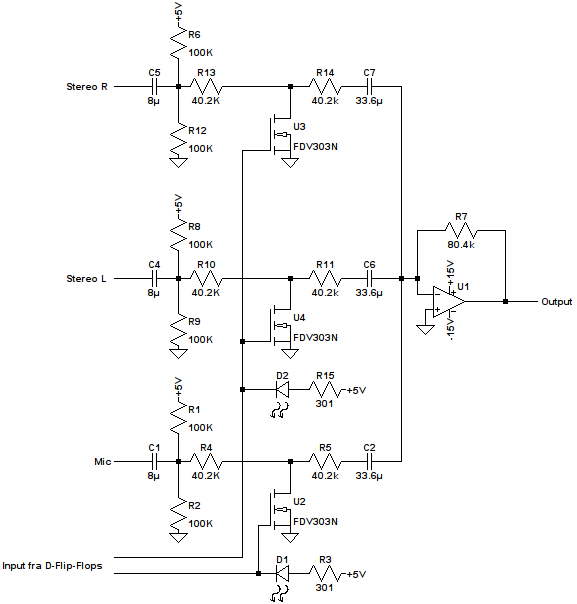
\includegraphics[scale=0.8]{maalerapporter/indgangsvaelger/indgangvaelger_ltspice_diagram.png}
\caption{Diagram over kredsløbet der testes.}
\label{diagram_simulering}
\end{figure}

\subsection*{Måleopstilling}
Måleopstillingerne er vist på figur \ref{fig:indgang:maaleop-thd} .

\begin{figure}[h]
\centering
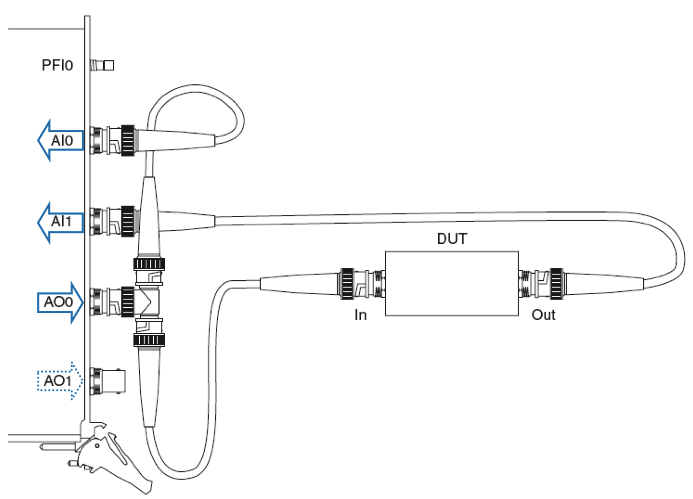
\includegraphics[scale=0.4]{maalerapporter/indgangsvaelger/maaleopstilling-thd-forforstaerker.png}
\caption{Måleopstilling for forstærkning-, frekvensgang- og forvrængningsmåling}
\label{fig:indgang:maaleop-thd}
\end{figure}


\subsection*{Anvendt udstyr}

\begin{table}[h]
\centering
\begin{tabular}{l|c|l}
\hline\hline
Instrument & AAU-nr. & Fabrikant, type m.v. \\
\hline\hline
Spændingsforsyning & 39897 & HAMEG HM7042 \\[4pt]
Spændingsforsyning & 33901 & HAMEG HM7042 \\[4pt]
Multimeter & 08518 & Fluke and Philips FLUKE 37 \\[4pt]
Audioanalysator & 76986 & National Instruments NI-PCI-4461 \\
\hline\hline
\end{tabular}
\label{tab:indgang:maaleudstyr_forforstaerker}
\end{table}

\subsection*{Måleprocedure}
\begin{enumerate}
\item En spændingsforsyning indstilles til $\pm15~V$ (indstilles med multimeteret) og tilsluttes.
\item En spændingsforsyning indstilles til 5 V (indstilles med multimeteret) og tilsluttes.
\item Testobjektet tilsluttes som på figur \ref{fig:indgang:maaleop-thd}
\item Kanalen der måles på, indstilles ved hjælp af trykknappen.
\item Programmet $"$Swept Sine - Linear Response and Harmonic Distortion (DAQmx)$"$ startes
\item $"$Start frequency$"$ under Source settings sættes til 20 Hz
\item $"$Stop frequency$"$ under Source settings sættes til 20 kHz
\item $"$Amplitude$"$ under Source settings sættes til 2 V
\item $"$THD units$"$ sættes til \%
\item $"$AI Range$"$ for Stimulus channel sættes til $\pm$ 0,316 V\fixme{Check}
\item $"$AI Range$"$ for Respons channel sættes til $\pm$ 3,16 V\fixme{dem her}
\item $"$Sampling frequency$"$ sættes til 204,8 kHz
\end{enumerate}

\subsection*{Resultater}

THD blev målt for de forskellige opsætninger. Her er vist resultater for mikrofonindgangen ved forskellige indstillinger. Resten af resultaterne kan findes på CD'en\fixme{henvisning}. Frekvenssweep foretages ved 2 V.

THD uden opamp og uden transistore vises i figur \ref{fig:apind:uoput}.
\begin{figure}[h]
\centering
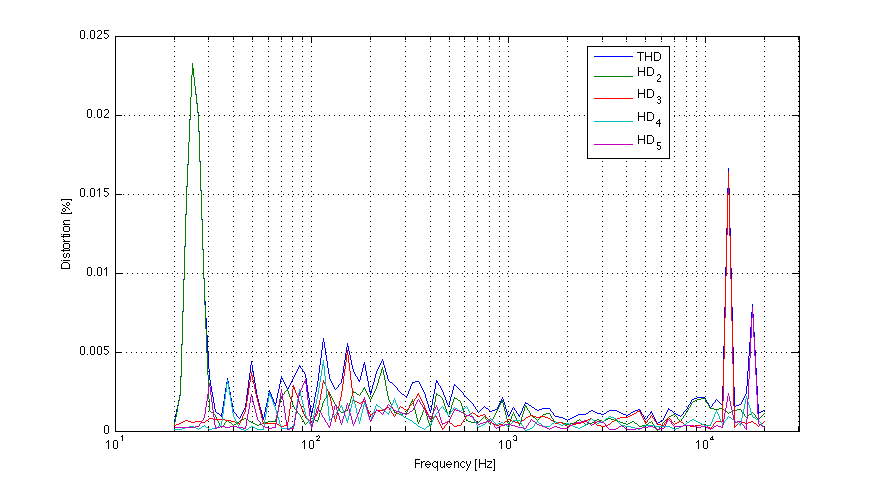
\includegraphics[width=\textwidth]{maalerapporter/indgangsvaelger/maalinger/2. gang/ingen opamp 2V uden transistor thd.png}
\caption{THD uden opamp og uden transistore}
\label{fig:apind:uoput}
\end{figure}

THD uden opamp men med transistore vises i figur \ref{fig:apind:uopmt}.
\begin{figure}[h]
\centering
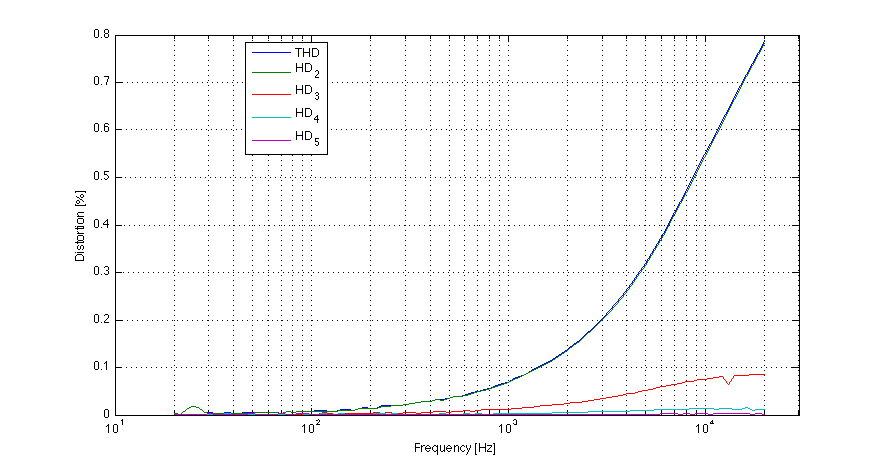
\includegraphics[width=\textwidth]{maalerapporter/indgangsvaelger/maalinger/2. gang/ingen opamp 2V med transistor thd.png}
\caption{THD uden opamp men med transistore}
\label{fig:apind:uopmt}
\end{figure}

THD uden opamp men med transistore vises i figur \ref{fig:apind:uopmt}.
\begin{figure}[h]
\centering
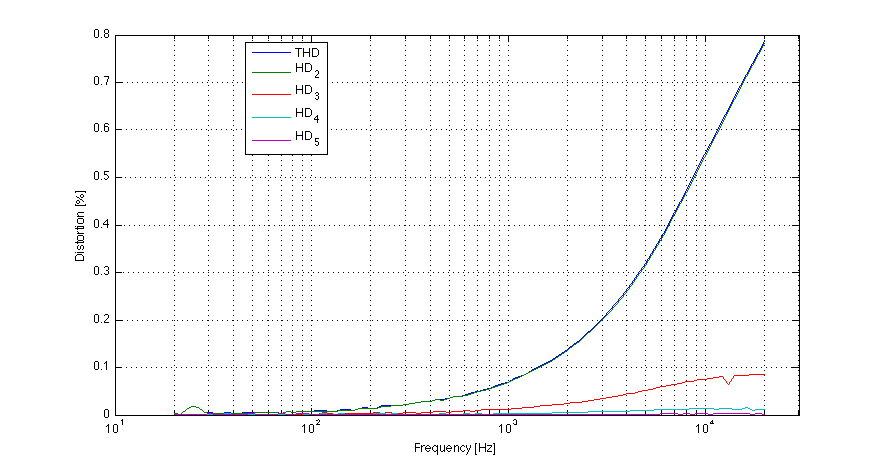
\includegraphics[width=\textwidth]{maalerapporter/indgangsvaelger/maalinger/2. gang/ingen opamp 2V med transistor thd.png}
\caption{THD uden opamp men med transistore}
\label{fig:apind:uopmt}
\end{figure}



Nogle resultater kan med fordel flyttes (eller kopieres) til rapporten – husk henvisning \\
Ofte angives tabeller i målejournalen og grafer i rapporten \\
Brug tabeller – resultater blandet med tekst bliver rodet\\
Datafiler bør (desuden) vedlægges rapporten på en CD – husk henvisning\\
Præcis formulering er vigtig!!\\
Angiv enheder - DC, RMS, amplitude, eller spids-spids værdier?\\

\subsection*{Måleusikkerheder}
Her angives væsentlige fejlkilder og usikkerheder i.f.b. med målingen. \\
Principielt skal man medtage alle usikkerheder og lave en samlet usikkerhedsberegning, men oftest nævnes kun de mest væsentlige. \\
Det er vigtigt at forklare uoverensstemmelser mellem beregnede, simulerede og målte data, men det hører hjemme i hovedrapporten – ikke i målejournalen. \\
I rapporten kan man evt. henvise til usikkerheder beskrevet i målejournalen.\\
Typiske årsager til måleunøjagtighed:\\
Måleinstrumenter påvirker (belaster) måleobjektet\\
Aflæsningsunøjagtighed\\
Analoge (antikke) viserinstrumenter	\\
Oscilloscop-cursor (pas på støj i ”auto-peak-peak”)\\
Støj, 50 Hz (100 Hz) brum, switch-mode spændingsforsyninger m.v.\\
Instrumentets unøjagtighed: Se manualen! \\
Multimetre: Frekvensafhængig måleusikkerhed \\
Oscilloscop: Både horisontal (lille) og vertikal usikkerhed\\\fixme{husk at ændre det her}
%\end{document}